% Options for packages loaded elsewhere
\PassOptionsToPackage{unicode}{hyperref}
\PassOptionsToPackage{hyphens}{url}
%
\documentclass[
]{article}
\usepackage{lmodern}
\usepackage{amsmath}
\usepackage{ifxetex,ifluatex}
\ifnum 0\ifxetex 1\fi\ifluatex 1\fi=0 % if pdftex
  \usepackage[T1]{fontenc}
  \usepackage[utf8]{inputenc}
  \usepackage{textcomp} % provide euro and other symbols
  \usepackage{amssymb}
\else % if luatex or xetex
  \usepackage{unicode-math}
  \defaultfontfeatures{Scale=MatchLowercase}
  \defaultfontfeatures[\rmfamily]{Ligatures=TeX,Scale=1}
\fi
% Use upquote if available, for straight quotes in verbatim environments
\IfFileExists{upquote.sty}{\usepackage{upquote}}{}
\IfFileExists{microtype.sty}{% use microtype if available
  \usepackage[]{microtype}
  \UseMicrotypeSet[protrusion]{basicmath} % disable protrusion for tt fonts
}{}
\makeatletter
\@ifundefined{KOMAClassName}{% if non-KOMA class
  \IfFileExists{parskip.sty}{%
    \usepackage{parskip}
  }{% else
    \setlength{\parindent}{0pt}
    \setlength{\parskip}{6pt plus 2pt minus 1pt}}
}{% if KOMA class
  \KOMAoptions{parskip=half}}
\makeatother
\usepackage{xcolor}
\IfFileExists{xurl.sty}{\usepackage{xurl}}{} % add URL line breaks if available
\IfFileExists{bookmark.sty}{\usepackage{bookmark}}{\usepackage{hyperref}}
\hypersetup{
  pdftitle={Gestion de Portefeuille},
  pdfauthor={Paul Giraud , Kouamé YAO \& Loïc Turounet},
  hidelinks,
  pdfcreator={LaTeX via pandoc}}
\urlstyle{same} % disable monospaced font for URLs
\usepackage[margin=1in]{geometry}
\usepackage{color}
\usepackage{fancyvrb}
\newcommand{\VerbBar}{|}
\newcommand{\VERB}{\Verb[commandchars=\\\{\}]}
\DefineVerbatimEnvironment{Highlighting}{Verbatim}{commandchars=\\\{\}}
% Add ',fontsize=\small' for more characters per line
\usepackage{framed}
\definecolor{shadecolor}{RGB}{248,248,248}
\newenvironment{Shaded}{\begin{snugshade}}{\end{snugshade}}
\newcommand{\AlertTok}[1]{\textcolor[rgb]{0.94,0.16,0.16}{#1}}
\newcommand{\AnnotationTok}[1]{\textcolor[rgb]{0.56,0.35,0.01}{\textbf{\textit{#1}}}}
\newcommand{\AttributeTok}[1]{\textcolor[rgb]{0.77,0.63,0.00}{#1}}
\newcommand{\BaseNTok}[1]{\textcolor[rgb]{0.00,0.00,0.81}{#1}}
\newcommand{\BuiltInTok}[1]{#1}
\newcommand{\CharTok}[1]{\textcolor[rgb]{0.31,0.60,0.02}{#1}}
\newcommand{\CommentTok}[1]{\textcolor[rgb]{0.56,0.35,0.01}{\textit{#1}}}
\newcommand{\CommentVarTok}[1]{\textcolor[rgb]{0.56,0.35,0.01}{\textbf{\textit{#1}}}}
\newcommand{\ConstantTok}[1]{\textcolor[rgb]{0.00,0.00,0.00}{#1}}
\newcommand{\ControlFlowTok}[1]{\textcolor[rgb]{0.13,0.29,0.53}{\textbf{#1}}}
\newcommand{\DataTypeTok}[1]{\textcolor[rgb]{0.13,0.29,0.53}{#1}}
\newcommand{\DecValTok}[1]{\textcolor[rgb]{0.00,0.00,0.81}{#1}}
\newcommand{\DocumentationTok}[1]{\textcolor[rgb]{0.56,0.35,0.01}{\textbf{\textit{#1}}}}
\newcommand{\ErrorTok}[1]{\textcolor[rgb]{0.64,0.00,0.00}{\textbf{#1}}}
\newcommand{\ExtensionTok}[1]{#1}
\newcommand{\FloatTok}[1]{\textcolor[rgb]{0.00,0.00,0.81}{#1}}
\newcommand{\FunctionTok}[1]{\textcolor[rgb]{0.00,0.00,0.00}{#1}}
\newcommand{\ImportTok}[1]{#1}
\newcommand{\InformationTok}[1]{\textcolor[rgb]{0.56,0.35,0.01}{\textbf{\textit{#1}}}}
\newcommand{\KeywordTok}[1]{\textcolor[rgb]{0.13,0.29,0.53}{\textbf{#1}}}
\newcommand{\NormalTok}[1]{#1}
\newcommand{\OperatorTok}[1]{\textcolor[rgb]{0.81,0.36,0.00}{\textbf{#1}}}
\newcommand{\OtherTok}[1]{\textcolor[rgb]{0.56,0.35,0.01}{#1}}
\newcommand{\PreprocessorTok}[1]{\textcolor[rgb]{0.56,0.35,0.01}{\textit{#1}}}
\newcommand{\RegionMarkerTok}[1]{#1}
\newcommand{\SpecialCharTok}[1]{\textcolor[rgb]{0.00,0.00,0.00}{#1}}
\newcommand{\SpecialStringTok}[1]{\textcolor[rgb]{0.31,0.60,0.02}{#1}}
\newcommand{\StringTok}[1]{\textcolor[rgb]{0.31,0.60,0.02}{#1}}
\newcommand{\VariableTok}[1]{\textcolor[rgb]{0.00,0.00,0.00}{#1}}
\newcommand{\VerbatimStringTok}[1]{\textcolor[rgb]{0.31,0.60,0.02}{#1}}
\newcommand{\WarningTok}[1]{\textcolor[rgb]{0.56,0.35,0.01}{\textbf{\textit{#1}}}}
\usepackage{graphicx}
\makeatletter
\def\maxwidth{\ifdim\Gin@nat@width>\linewidth\linewidth\else\Gin@nat@width\fi}
\def\maxheight{\ifdim\Gin@nat@height>\textheight\textheight\else\Gin@nat@height\fi}
\makeatother
% Scale images if necessary, so that they will not overflow the page
% margins by default, and it is still possible to overwrite the defaults
% using explicit options in \includegraphics[width, height, ...]{}
\setkeys{Gin}{width=\maxwidth,height=\maxheight,keepaspectratio}
% Set default figure placement to htbp
\makeatletter
\def\fps@figure{htbp}
\makeatother
\setlength{\emergencystretch}{3em} % prevent overfull lines
\providecommand{\tightlist}{%
  \setlength{\itemsep}{0pt}\setlength{\parskip}{0pt}}
\setcounter{secnumdepth}{-\maxdimen} % remove section numbering
\usepackage[utf8]{inputenc}
\usepackage{booktabs}
\usepackage{longtable}
\usepackage{array}
\usepackage{multirow}
\usepackage{wrapfig}
\usepackage{float}
\usepackage{colortbl}
\usepackage{pdflscape}
\usepackage{tabu}
\usepackage{threeparttable}
\usepackage{threeparttablex}
\usepackage[normalem]{ulem}
\usepackage{makecell}
\usepackage{xcolor}
\ifluatex
  \usepackage{selnolig}  % disable illegal ligatures
\fi

\title{Gestion de Portefeuille}
\usepackage{etoolbox}
\makeatletter
\providecommand{\subtitle}[1]{% add subtitle to \maketitle
  \apptocmd{\@title}{\par {\large #1 \par}}{}{}
}
\makeatother
\subtitle{TP-2: Droite de Marchés des Capitaux}
\author{Paul Giraud , Kouamé YAO \& Loïc Turounet}
\date{Version: 27 fév 2022}

\begin{document}
\maketitle

\hypertarget{donnuxe9es}{%
\section{Données}\label{donnuxe9es}}

\hypertarget{suxe9ries-de-rendement-quotidien-pour-11-valeurs}{%
\subsection{Séries de rendement quotidien pour 11
valeurs:}\label{suxe9ries-de-rendement-quotidien-pour-11-valeurs}}

\begin{Shaded}
\begin{Highlighting}[]
\NormalTok{daily.ret.file }\OtherTok{\textless{}{-}} \FunctionTok{file.path}\NormalTok{(}\FunctionTok{get.data.folder}\NormalTok{(), }\StringTok{"daily.ret.rda"}\NormalTok{)}
\FunctionTok{load}\NormalTok{(daily.ret.file)}
\FunctionTok{kable}\NormalTok{(}\FunctionTok{table.Stats}\NormalTok{(daily.ret), }\StringTok{"latex"}\NormalTok{, }\AttributeTok{booktabs=}\NormalTok{T) }\SpecialCharTok{\%\textgreater{}\%} \FunctionTok{kable\_styling}\NormalTok{(}\AttributeTok{latex\_options=}\StringTok{"scale\_down"}\NormalTok{)}
\end{Highlighting}
\end{Shaded}

\begin{table}
\centering
\resizebox{\linewidth}{!}{
\begin{tabular}{lrrrrrrrrrrr}
\toprule
  & AAPL & AMZN & MSFT & F & SPY & QQQ & XOM & MMM & HD & PG & KO\\
\midrule
Observations & 3308.0000 & 3308.0000 & 3308.0000 & 3308.0000 & 3308.0000 & 3308.0000 & 3308.0000 & 3308.0000 & 3308.0000 & 3308.0000 & 3308.0000\\
NAs & 0.0000 & 0.0000 & 0.0000 & 0.0000 & 0.0000 & 0.0000 & 0.0000 & 0.0000 & 0.0000 & 0.0000 & 0.0000\\
Minimum & -0.1792 & -0.1278 & -0.1171 & -0.2500 & -0.0984 & -0.0896 & -0.1395 & -0.1295 & -0.0822 & -0.0790 & -0.0867\\
Quartile 1 & -0.0077 & -0.0094 & -0.0073 & -0.0103 & -0.0038 & -0.0047 & -0.0068 & -0.0055 & -0.0067 & -0.0046 & -0.0047\\
Median & 0.0010 & 0.0008 & 0.0005 & 0.0000 & 0.0006 & 0.0010 & 0.0001 & 0.0008 & 0.0006 & 0.0004 & 0.0007\\
\addlinespace
Arithmetic Mean & 0.0012 & 0.0015 & 0.0008 & 0.0005 & 0.0004 & 0.0006 & 0.0001 & 0.0004 & 0.0008 & 0.0004 & 0.0005\\
Geometric Mean & 0.0010 & 0.0012 & 0.0006 & 0.0001 & 0.0003 & 0.0005 & 0.0000 & 0.0003 & 0.0006 & 0.0003 & 0.0004\\
Quartile 3 & 0.0112 & 0.0123 & 0.0088 & 0.0106 & 0.0056 & 0.0070 & 0.0073 & 0.0070 & 0.0082 & 0.0055 & 0.0059\\
Maximum & 0.1390 & 0.2695 & 0.1860 & 0.2952 & 0.1452 & 0.1216 & 0.1719 & 0.0988 & 0.1407 & 0.1021 & 0.1388\\
SE Mean & 0.0003 & 0.0004 & 0.0003 & 0.0005 & 0.0002 & 0.0002 & 0.0003 & 0.0002 & 0.0003 & 0.0002 & 0.0002\\
\addlinespace
LCL Mean (0.95) & 0.0005 & 0.0006 & 0.0002 & -0.0005 & 0.0000 & 0.0002 & -0.0004 & -0.0001 & 0.0002 & 0.0000 & 0.0001\\
UCL Mean (0.95) & 0.0019 & 0.0023 & 0.0013 & 0.0014 & 0.0008 & 0.0011 & 0.0006 & 0.0009 & 0.0013 & 0.0007 & 0.0009\\
Variance & 0.0004 & 0.0006 & 0.0003 & 0.0007 & 0.0001 & 0.0002 & 0.0002 & 0.0002 & 0.0003 & 0.0001 & 0.0001\\
Stdev & 0.0196 & 0.0243 & 0.0170 & 0.0266 & 0.0121 & 0.0130 & 0.0150 & 0.0140 & 0.0162 & 0.0109 & 0.0113\\
Skewness & -0.2151 & 1.4889 & 0.4319 & 0.7627 & 0.1379 & -0.0084 & 0.4199 & -0.3815 & 0.5114 & 0.0555 & 0.5004\\
\addlinespace
Kurtosis & 6.2706 & 16.8872 & 10.2176 & 20.9458 & 15.2824 & 7.3976 & 15.4203 & 7.3856 & 6.4641 & 8.1017 & 14.3236\\
\bottomrule
\end{tabular}}
\end{table}

\hypertarget{rendement-annuel-moyen}{%
\subsection{Rendement annuel moyen:}\label{rendement-annuel-moyen}}

\begin{Shaded}
\begin{Highlighting}[]
\FunctionTok{kable}\NormalTok{(}\DecValTok{252}\SpecialCharTok{*}\DecValTok{100}\SpecialCharTok{*}\FunctionTok{colMeans}\NormalTok{(daily.ret), }\StringTok{"latex"}\NormalTok{, }\AttributeTok{booktabs=}\NormalTok{T, }\AttributeTok{digits=}\DecValTok{1}\NormalTok{, }\AttributeTok{col.names=}\FunctionTok{c}\NormalTok{(}\StringTok{"Rendement (\%)"}\NormalTok{),}
      \AttributeTok{caption=}\StringTok{"Rendement annuel moyen"}\NormalTok{)}
\end{Highlighting}
\end{Shaded}

\begin{table}

\caption{\label{tab:unnamed-chunk-2}Rendement annuel moyen}
\centering
\begin{tabular}[t]{lr}
\toprule
  & Rendement (\%)\\
\midrule
AAPL & 30.2\\
AMZN & 37.2\\
MSFT & 19.0\\
F & 11.4\\
SPY & 9.9\\
\addlinespace
QQQ & 15.3\\
XOM & 3.5\\
MMM & 9.9\\
HD & 19.2\\
PG & 9.3\\
\addlinespace
KO & 12.5\\
\bottomrule
\end{tabular}
\end{table}

\hypertarget{matrice-de-corruxe9lation-des-rendements}{%
\subsection{Matrice de corrélation des
rendements:}\label{matrice-de-corruxe9lation-des-rendements}}

\begin{Shaded}
\begin{Highlighting}[]
\NormalTok{correl }\OtherTok{\textless{}{-}} \FunctionTok{cor}\NormalTok{(daily.ret)}
\NormalTok{correl[}\FunctionTok{lower.tri}\NormalTok{(correl)] }\OtherTok{\textless{}{-}} \ConstantTok{NA}
\FunctionTok{options}\NormalTok{(}\AttributeTok{knitr.kable.NA =} \StringTok{\textquotesingle{}\textquotesingle{}}\NormalTok{)}
\FunctionTok{kable}\NormalTok{(correl, }\StringTok{"latex"}\NormalTok{, }\AttributeTok{booktabs=}\NormalTok{T, }\AttributeTok{digits=}\DecValTok{2}\NormalTok{, }\AttributeTok{caption=}\StringTok{"Corrélation des rendements quotidiens"}\NormalTok{) }\SpecialCharTok{\%\textgreater{}\%}
\FunctionTok{kable\_styling}\NormalTok{(}\AttributeTok{latex\_options=}\StringTok{"scale\_down"}\NormalTok{)}
\end{Highlighting}
\end{Shaded}

\begin{table}

\caption{\label{tab:unnamed-chunk-3}Corrélation des rendements quotidiens}
\centering
\resizebox{\linewidth}{!}{
\begin{tabular}[t]{lrrrrrrrrrrr}
\toprule
  & AAPL & AMZN & MSFT & F & SPY & QQQ & XOM & MMM & HD & PG & KO\\
\midrule
AAPL & 1 & 0.46 & 0.49 & 0.37 & 0.61 & 0.75 & 0.40 & 0.45 & 0.42 & 0.32 & 0.32\\
AMZN &  & 1.00 & 0.50 & 0.33 & 0.56 & 0.66 & 0.39 & 0.41 & 0.44 & 0.27 & 0.30\\
MSFT &  &  & 1.00 & 0.39 & 0.71 & 0.76 & 0.53 & 0.53 & 0.49 & 0.44 & 0.46\\
F &  &  &  & 1.00 & 0.56 & 0.53 & 0.37 & 0.44 & 0.46 & 0.30 & 0.31\\
SPY &  &  &  &  & 1.00 & 0.92 & 0.77 & 0.75 & 0.71 & 0.62 & 0.60\\
\addlinespace
QQQ &  &  &  &  &  & 1.00 & 0.64 & 0.69 & 0.66 & 0.52 & 0.52\\
XOM &  &  &  &  &  &  & 1.00 & 0.60 & 0.47 & 0.52 & 0.49\\
MMM &  &  &  &  &  &  &  & 1.00 & 0.55 & 0.50 & 0.47\\
HD &  &  &  &  &  &  &  &  & 1.00 & 0.45 & 0.44\\
PG &  &  &  &  &  &  &  &  &  & 1.00 & 0.57\\
\addlinespace
KO &  &  &  &  &  &  &  &  &  &  & 1.00\\
\bottomrule
\end{tabular}}
\end{table}

\hypertarget{droite-de-marchuxe9-des-capitaux-capital-market-line}{%
\section{Droite de Marché des Capitaux (Capital Market
Line)}\label{droite-de-marchuxe9-des-capitaux-capital-market-line}}

\begin{itemize}
\tightlist
\item
  A partir des calculs présentés en cours, mettre en oeuvre une méthode
  numérique pour déterminer le portefeuille tangent quand les poids des
  actifs risqués sont contraints à être positifs: \(w_i >= 0\).
\end{itemize}

Pour déterminer le portefeuille nous devons calculer le portefeuille sur
frontière efficiente qui maximise le ratio de Sharpe càd: \[
\begin{aligned}
    \mbox{max}_w \ \  &  \frac{w^T \mu - r_f}{(w^T \Sigma w)^{\frac{1}{2}}} \\
    \mbox{s.t.} & \\
    & \mathbf{1}^T w  = 1
\end{aligned}
\] Solution: \[
w = \frac{\Sigma^{-1}(\mu - r_f  \mathbf{1})}{\mathbf{1}^T\Sigma^{-1}(\mu - r_f \mathbf{1})}
\]

Dans un premier temps nous allons voir la frontière en utilisant le
modèle de Markowitz: \[
\begin{aligned}
    \mbox{min}\ \  &  w^T \Sigma w \\
    \mbox{s.t.} & \\
    & \mu^T w = \mu^* \\
    & \mathbf{1}^T w  = 1
\end{aligned}
\]

\hypertarget{calcul-de-la-frontiuxe8re-de-marchuxe9-long}{%
\subsubsection{Calcul de la frontière de marché
(Long)}\label{calcul-de-la-frontiuxe8re-de-marchuxe9-long}}

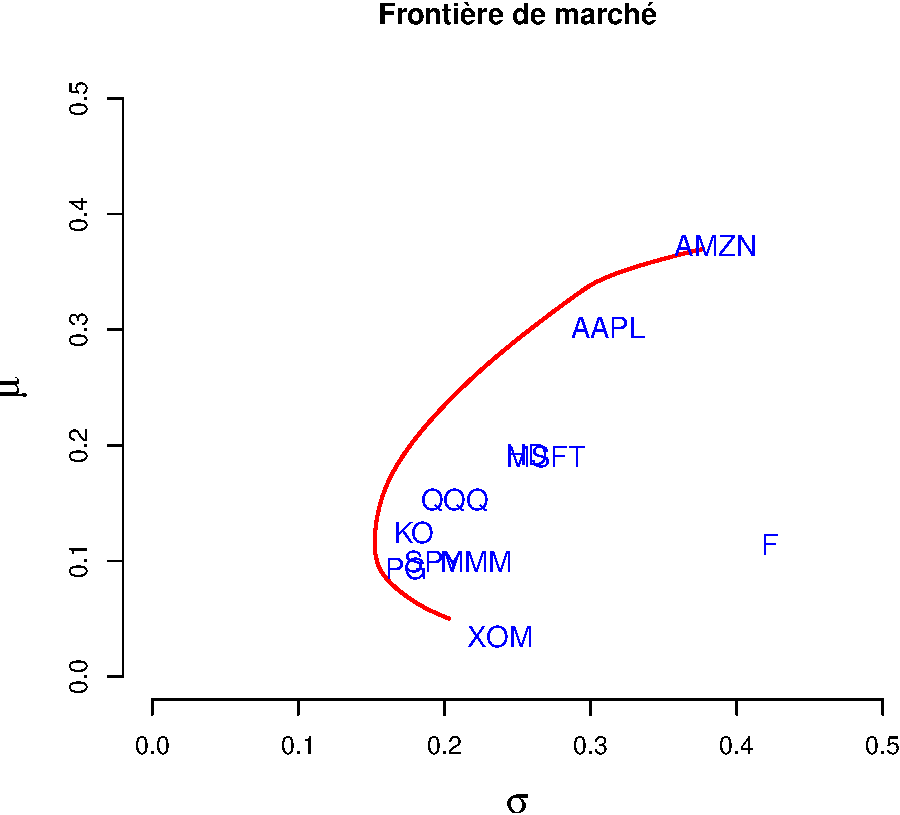
\includegraphics{TP-2_files/figure-latex/unnamed-chunk-5-1.pdf}

Nous avons imposé que les poids des actifs soient contraints à être
positifs, donc que nous ne pouvions pas vendre à découvert ces actifs.
Nous pouvons vérifier cela dans l'allocation le long de la frontière de
marché.

\hypertarget{allocation-le-long-de-la-frontiuxe8re}{%
\subsubsection{Allocation le long de la
frontière}\label{allocation-le-long-de-la-frontiuxe8re}}

\begin{Shaded}
\begin{Highlighting}[]
\FunctionTok{chart.StackedBar}\NormalTok{(sol[, }\DecValTok{3}\SpecialCharTok{+}\FunctionTok{seq\_along}\NormalTok{(mu)], }\AttributeTok{xaxis.labels=}\FunctionTok{round}\NormalTok{(sol[,}\StringTok{"stdev"}\NormalTok{],}\DecValTok{2}\NormalTok{), }
                 \AttributeTok{xlab=}\StringTok{"SD Portefeuille"}\NormalTok{, }\AttributeTok{ylab=}\StringTok{"Allocation le long de la frontière"}\NormalTok{)}
\end{Highlighting}
\end{Shaded}

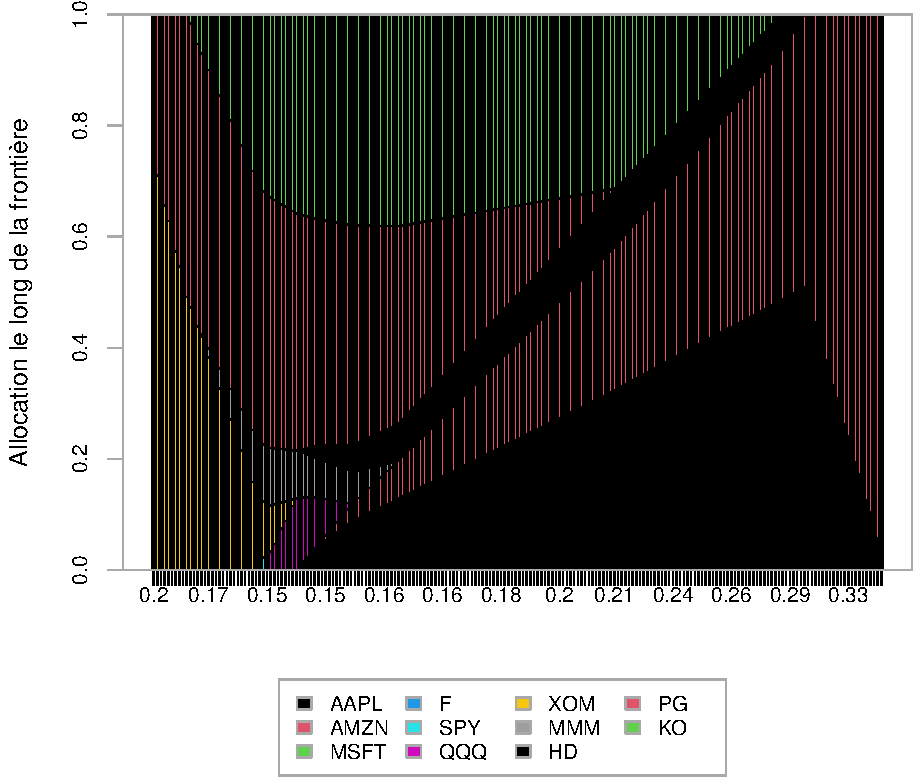
\includegraphics{TP-2_files/figure-latex/unnamed-chunk-6-1.pdf}

\hypertarget{calcul-de-la-frontiuxe8re-long-en-ajoutant-un-actif-sans-risque-pour-obtenir-le-portefeuille-tangent.}{%
\subsubsection{Calcul de la Frontière (Long) en ajoutant un actif sans
risque pour obtenir le portefeuille
tangent.}\label{calcul-de-la-frontiuxe8re-long-en-ajoutant-un-actif-sans-risque-pour-obtenir-le-portefeuille-tangent.}}

Maintenant pour obtenir le portefeuille tangent nous allons ajouter un
actif sans risque au portefeuille :

\begin{Shaded}
\begin{Highlighting}[]
\NormalTok{sol.with.rf }\OtherTok{\textless{}{-}} \ConstantTok{NULL}
\ControlFlowTok{for}\NormalTok{(mu.star }\ControlFlowTok{in} \FunctionTok{seq}\NormalTok{(}\AttributeTok{from=}\NormalTok{rf, }\AttributeTok{to=}\FloatTok{1.3}\NormalTok{, }\AttributeTok{length.out=}\DecValTok{200}\NormalTok{))\{}
\NormalTok{  tmp }\OtherTok{\textless{}{-}} \FunctionTok{matrix}\NormalTok{(}\FunctionTok{c}\NormalTok{(mu.star, (mu.star }\SpecialCharTok{{-}}\NormalTok{ rf)}\SpecialCharTok{/}\NormalTok{sharpe.max , sharpe.max, (mu.star }\SpecialCharTok{{-}}\NormalTok{ rf)}\SpecialCharTok{*}\NormalTok{w.tangent), }\AttributeTok{nrow=}\DecValTok{1}\NormalTok{)}
  \ControlFlowTok{if}\NormalTok{(}\FunctionTok{is.null}\NormalTok{(sol.with.rf)) \{}
\NormalTok{    sol.with.rf }\OtherTok{\textless{}{-}}\NormalTok{ tmp  }
\NormalTok{  \} }\ControlFlowTok{else}\NormalTok{ \{}
\NormalTok{    sol.with.rf }\OtherTok{\textless{}{-}} \FunctionTok{rbind}\NormalTok{(sol.with.rf, tmp)}
\NormalTok{  \}}
\NormalTok{\}}
\FunctionTok{dimnames}\NormalTok{(w.tangent)}\OtherTok{\textless{}{-}} \FunctionTok{list}\NormalTok{(tickers)}
\NormalTok{sigma.tangent }\OtherTok{\textless{}{-}} \FunctionTok{sqrt}\NormalTok{(}\FunctionTok{t}\NormalTok{(w.tangent) }\SpecialCharTok{\%*\%}\NormalTok{ Sigma }\SpecialCharTok{\%*\%}\NormalTok{ w.tangent)}
\FunctionTok{colnames}\NormalTok{(sol.with.rf) }\OtherTok{\textless{}{-}} \FunctionTok{c}\NormalTok{(}\StringTok{"mu"}\NormalTok{, }\StringTok{"stdev"}\NormalTok{, }\StringTok{"Sharpe"}\NormalTok{, tickers)}
\FunctionTok{colnames}\NormalTok{(sol) }\OtherTok{\textless{}{-}} \FunctionTok{c}\NormalTok{(}\StringTok{"mu"}\NormalTok{, }\StringTok{"stdev"}\NormalTok{, }\StringTok{"Sharpe"}\NormalTok{, tickers)}
\end{Highlighting}
\end{Shaded}

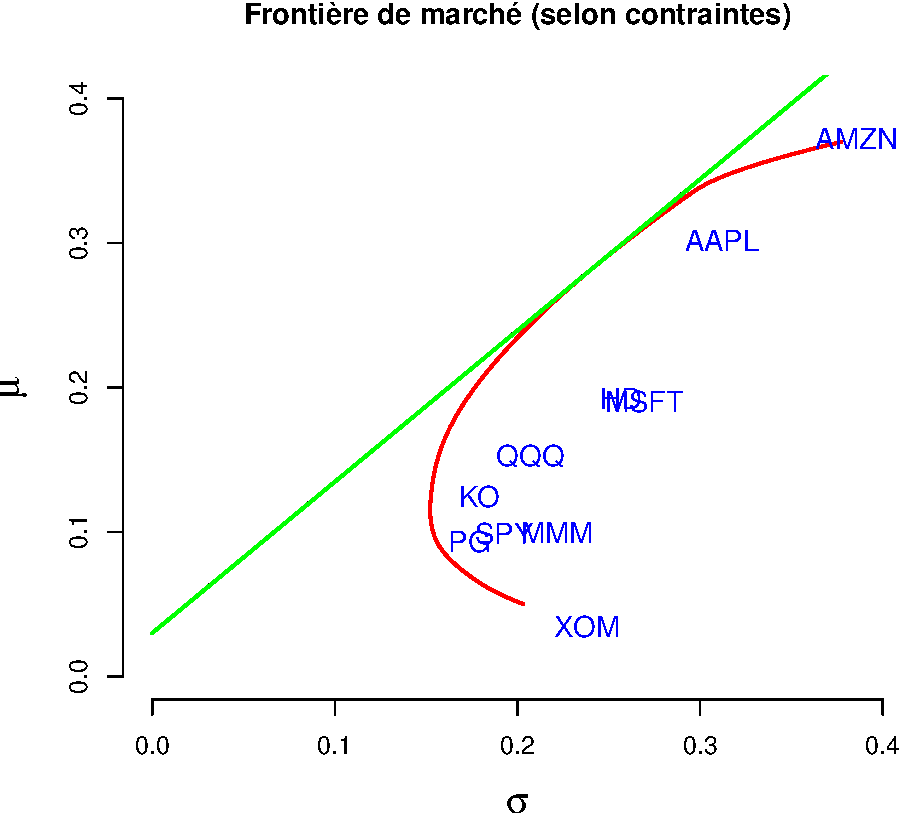
\includegraphics{TP-2_files/figure-latex/unnamed-chunk-8-1.pdf}

\hypertarget{allocation-le-long-de-la-droite-tangente}{%
\subsubsection{Allocation le long de la droite
tangente}\label{allocation-le-long-de-la-droite-tangente}}

\begin{Shaded}
\begin{Highlighting}[]
\NormalTok{cash }\OtherTok{\textless{}{-}} \DecValTok{1}\SpecialCharTok{{-}}\FunctionTok{rowSums}\NormalTok{(sol.with.rf[,}\DecValTok{3}\SpecialCharTok{+}\FunctionTok{seq\_along}\NormalTok{(mu)])}
\NormalTok{alloc }\OtherTok{\textless{}{-}} \FunctionTok{cbind}\NormalTok{(cash, sol.with.rf[,}\DecValTok{3}\SpecialCharTok{+}\FunctionTok{seq\_along}\NormalTok{(mu)] )}

\FunctionTok{chart.StackedBar}\NormalTok{(alloc, }\AttributeTok{xaxis.labels=}\FunctionTok{round}\NormalTok{(sol.with.rf[,}\StringTok{"stdev"}\NormalTok{],}\DecValTok{2}\NormalTok{), }
                 \AttributeTok{xlab=}\StringTok{"SD Portefeuille"}\NormalTok{, }\AttributeTok{ylab=}\StringTok{"Allocation le long de la droite tangent"}\NormalTok{)}
\end{Highlighting}
\end{Shaded}

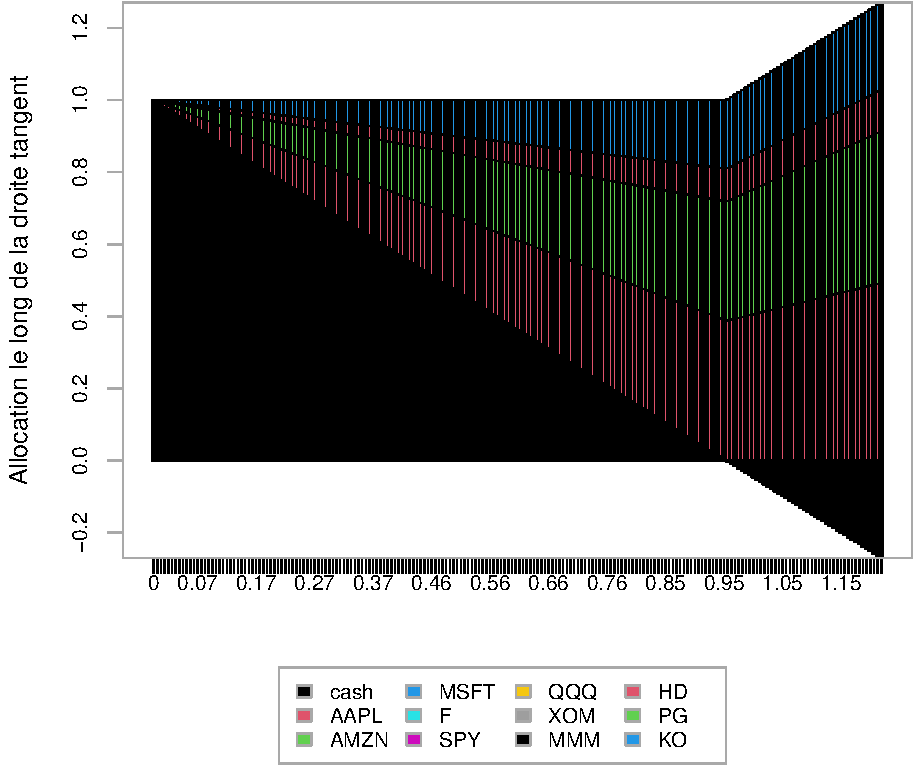
\includegraphics{TP-2_files/figure-latex/unnamed-chunk-9-1.pdf}

\hypertarget{composition-du-portefeuille-tangent}{%
\subsubsection{Composition du portefeuille
tangent}\label{composition-du-portefeuille-tangent}}

Nous pouvons remarquer d'après la table de composition du portefeuille
tangent que nous n'avons pas besoin seulement de 4 titres différents
pour le former. Nous pouvons voir que pour la participation pour Amazon
ou Apple est élevé. Un investisseur pourrait préférer ne pas investir
plus qu'un certain seuil dans un seul et même titre. Nous allons par
exemple dans la suite contraindre nos poids à ne pas dépasser 20 \%.

\begin{Shaded}
\begin{Highlighting}[]
\FunctionTok{kable}\NormalTok{(w.tangent}\SpecialCharTok{*}\DecValTok{100}\NormalTok{, }\AttributeTok{booktabs=}\NormalTok{T, }\AttributeTok{digits=}\DecValTok{2}\NormalTok{, }\AttributeTok{col.names =} \StringTok{"Proportion (\%)"}\NormalTok{,}
      \AttributeTok{caption=}\StringTok{"Composition du portefeuille tangent"}\NormalTok{)}
\end{Highlighting}
\end{Shaded}

\begin{table}

\caption{\label{tab:unnamed-chunk-10}Composition du portefeuille tangent}
\centering
\begin{tabular}[t]{lr}
\toprule
  & Proportion (\%)\\
\midrule
AAPL & 38.76\\
AMZN & 33.11\\
MSFT & 0.00\\
F & 0.00\\
SPY & 0.00\\
\addlinespace
QQQ & 0.00\\
XOM & 0.00\\
MMM & 0.00\\
HD & 9.07\\
PG & 0.00\\
\addlinespace
KO & 19.06\\
\bottomrule
\end{tabular}
\end{table}

Nous allons refaire les mêmes calcul en ajoutant des contraintes
supplémentaires qui nous semblent pertinentes

\hypertarget{pas-plus-de-20-de-lactif-risquuxe9-allouuxe9-uxe0-un-seul-titre}{%
\subsection{Pas plus de 20\% de l'actif risqué alloué à un seul
titre}\label{pas-plus-de-20-de-lactif-risquuxe9-allouuxe9-uxe0-un-seul-titre}}

\hypertarget{calcul-de-la-frontiuxe8re-de-marchuxe9-long-1}{%
\subsubsection{Calcul de la frontière de marché
(Long)}\label{calcul-de-la-frontiuxe8re-de-marchuxe9-long-1}}

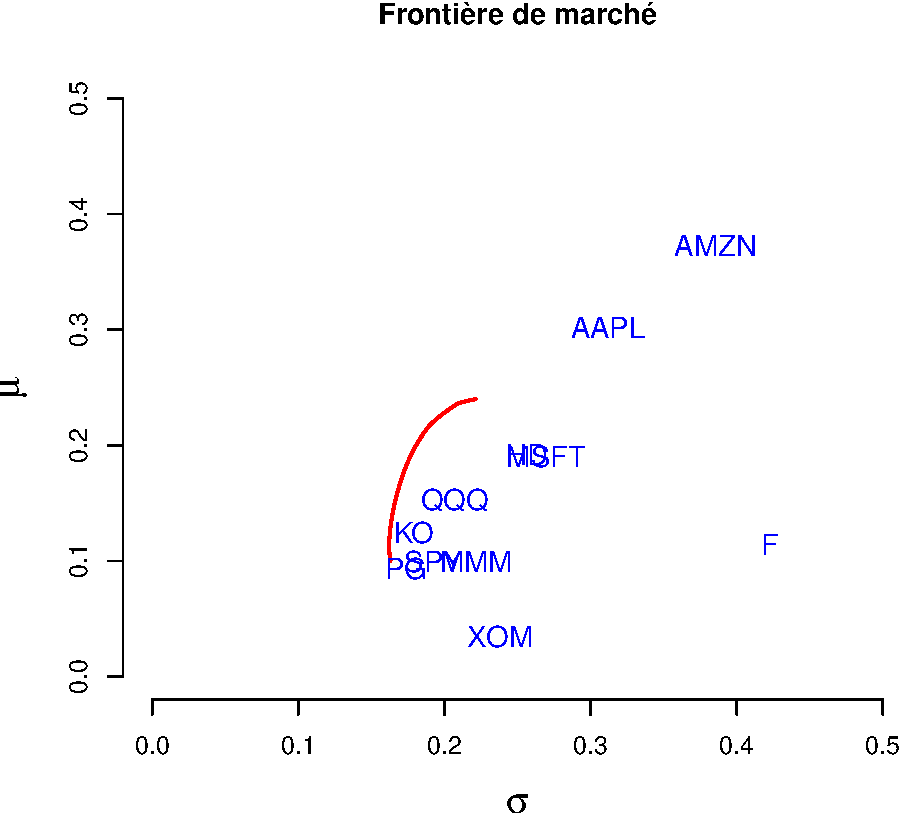
\includegraphics{TP-2_files/figure-latex/unnamed-chunk-12-1.pdf}

\hypertarget{calcul-du-portefeuille-tangent.}{%
\subsubsection{Calcul du portefeuille
tangent.}\label{calcul-du-portefeuille-tangent.}}

\begin{Shaded}
\begin{Highlighting}[]
\NormalTok{sol.with.rf }\OtherTok{\textless{}{-}} \ConstantTok{NULL}
\ControlFlowTok{for}\NormalTok{(mu.star }\ControlFlowTok{in} \FunctionTok{seq}\NormalTok{(}\AttributeTok{from=}\NormalTok{rf, }\AttributeTok{to=}\FloatTok{1.3}\NormalTok{, }\AttributeTok{length.out=}\DecValTok{200}\NormalTok{))\{}
\NormalTok{  tmp }\OtherTok{\textless{}{-}} \FunctionTok{matrix}\NormalTok{(}\FunctionTok{c}\NormalTok{(mu.star, (mu.star }\SpecialCharTok{{-}}\NormalTok{ rf)}\SpecialCharTok{/}\NormalTok{sharpe.max , sharpe.max, (mu.star }\SpecialCharTok{{-}}\NormalTok{ rf)}\SpecialCharTok{*}\NormalTok{w.tangent), }\AttributeTok{nrow=}\DecValTok{1}\NormalTok{)}
  \ControlFlowTok{if}\NormalTok{(}\FunctionTok{is.null}\NormalTok{(sol.with.rf)) \{}
\NormalTok{    sol.with.rf }\OtherTok{\textless{}{-}}\NormalTok{ tmp  }
\NormalTok{  \} }\ControlFlowTok{else}\NormalTok{ \{}
\NormalTok{    sol.with.rf }\OtherTok{\textless{}{-}} \FunctionTok{rbind}\NormalTok{(sol.with.rf, tmp)}
\NormalTok{  \}}
\NormalTok{\}}
\FunctionTok{dimnames}\NormalTok{(w.tangent)}\OtherTok{\textless{}{-}} \FunctionTok{list}\NormalTok{(tickers)}
\NormalTok{sigma.tangent }\OtherTok{\textless{}{-}} \FunctionTok{sqrt}\NormalTok{(}\FunctionTok{t}\NormalTok{(w.tangent) }\SpecialCharTok{\%*\%}\NormalTok{ Sigma }\SpecialCharTok{\%*\%}\NormalTok{ w.tangent)}
\FunctionTok{colnames}\NormalTok{(sol.with.rf) }\OtherTok{\textless{}{-}} \FunctionTok{c}\NormalTok{(}\StringTok{"mu"}\NormalTok{, }\StringTok{"stdev"}\NormalTok{, }\StringTok{"Sharpe"}\NormalTok{, tickers)}
\FunctionTok{colnames}\NormalTok{(sol) }\OtherTok{\textless{}{-}} \FunctionTok{c}\NormalTok{(}\StringTok{"mu"}\NormalTok{, }\StringTok{"stdev"}\NormalTok{, }\StringTok{"Sharpe"}\NormalTok{, tickers)}
\end{Highlighting}
\end{Shaded}

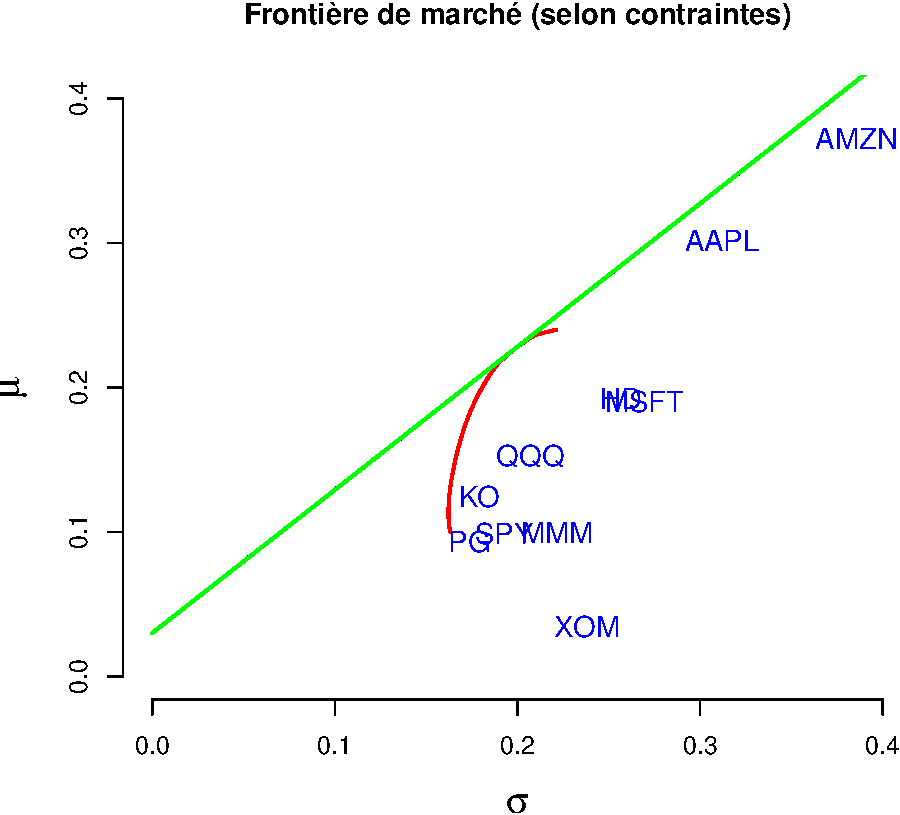
\includegraphics{TP-2_files/figure-latex/unnamed-chunk-14-1.pdf}

\hypertarget{allocation-le-long-de-la-droite-tangente-1}{%
\subsubsection{Allocation le long de la droite
tangente}\label{allocation-le-long-de-la-droite-tangente-1}}

\begin{Shaded}
\begin{Highlighting}[]
\NormalTok{cash }\OtherTok{\textless{}{-}} \DecValTok{1}\SpecialCharTok{{-}}\FunctionTok{rowSums}\NormalTok{(sol.with.rf[,}\DecValTok{3}\SpecialCharTok{+}\FunctionTok{seq\_along}\NormalTok{(mu)])}
\NormalTok{alloc }\OtherTok{\textless{}{-}} \FunctionTok{cbind}\NormalTok{(cash, sol.with.rf[,}\DecValTok{3}\SpecialCharTok{+}\FunctionTok{seq\_along}\NormalTok{(mu)] )}

\FunctionTok{chart.StackedBar}\NormalTok{(alloc, }\AttributeTok{xaxis.labels=}\FunctionTok{round}\NormalTok{(sol.with.rf[,}\StringTok{"stdev"}\NormalTok{],}\DecValTok{2}\NormalTok{), }
                 \AttributeTok{xlab=}\StringTok{"SD Portefeuille"}\NormalTok{, }\AttributeTok{ylab=}\StringTok{"Allocation le long de la droite tangent"}\NormalTok{)}
\end{Highlighting}
\end{Shaded}

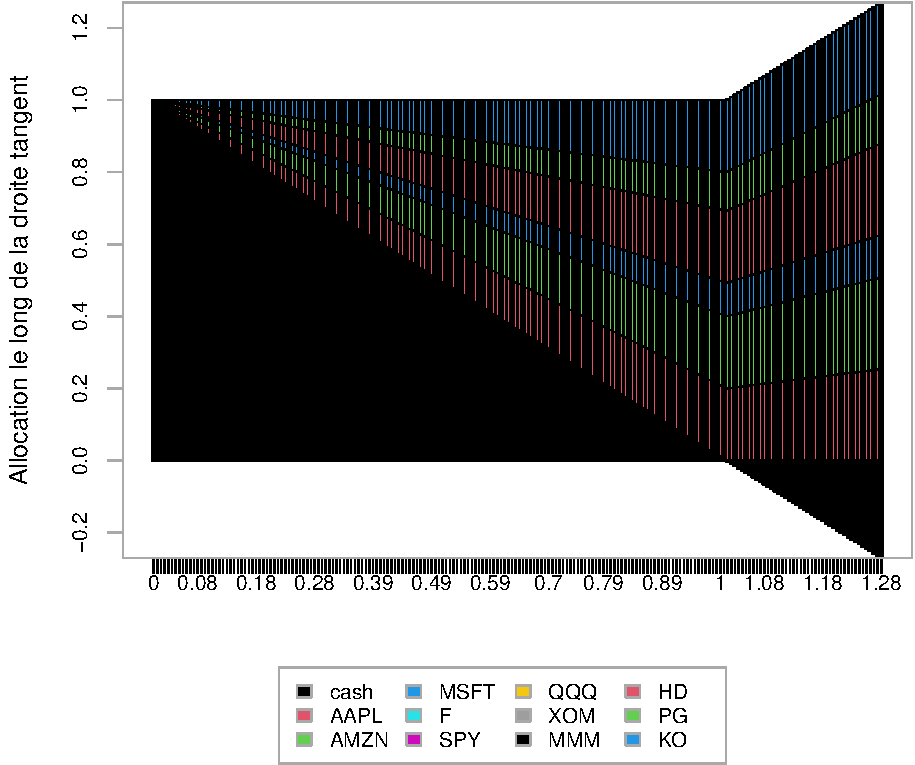
\includegraphics{TP-2_files/figure-latex/unnamed-chunk-15-1.pdf}

\hypertarget{composition-du-portefeuille-tangent-avec-contraintes}{%
\subsubsection{Composition du portefeuille tangent avec
contraintes}\label{composition-du-portefeuille-tangent-avec-contraintes}}

\begin{Shaded}
\begin{Highlighting}[]
\FunctionTok{kable}\NormalTok{(w.tangent}\SpecialCharTok{*}\DecValTok{100}\NormalTok{, }\AttributeTok{booktabs=}\NormalTok{T, }\AttributeTok{digits=}\DecValTok{2}\NormalTok{, }\AttributeTok{col.names =} \StringTok{"Proportion (\%)"}\NormalTok{,}
      \AttributeTok{caption=}\StringTok{"Composition du portefeuille tangent"}\NormalTok{)}
\end{Highlighting}
\end{Shaded}

\begin{table}

\caption{\label{tab:unnamed-chunk-16}Composition du portefeuille tangent}
\centering
\begin{tabular}[t]{lr}
\toprule
  & Proportion (\%)\\
\midrule
AAPL & 20.00\\
AMZN & 20.00\\
MSFT & 9.28\\
F & 0.00\\
SPY & 0.00\\
\addlinespace
QQQ & 0.00\\
XOM & 0.00\\
MMM & 0.00\\
HD & 20.00\\
PG & 10.72\\
\addlinespace
KO & 20.00\\
\bottomrule
\end{tabular}
\end{table}

\hypertarget{pas-plus-de-25-de-lactif-risquuxe9-allouuxe9-uxe0-un-seul-titre-et-investir-au-minimum-5-dans-chaque-titre}{%
\subsection{Pas plus de 25\% de l'actif risqué alloué à un seul titre et
investir au minimum 5\% dans chaque
titre}\label{pas-plus-de-25-de-lactif-risquuxe9-allouuxe9-uxe0-un-seul-titre-et-investir-au-minimum-5-dans-chaque-titre}}

Nous voulons maintenant diversifier au plus nos actifs. Pour cela, nous
voulons au minimum 3\% de chaque actif et ne pas leur allouer plus de
15\%.

\hypertarget{calcul-de-la-frontiuxe8re-de-marchuxe9-long-2}{%
\subsubsection{Calcul de la frontière de marché
(Long)}\label{calcul-de-la-frontiuxe8re-de-marchuxe9-long-2}}

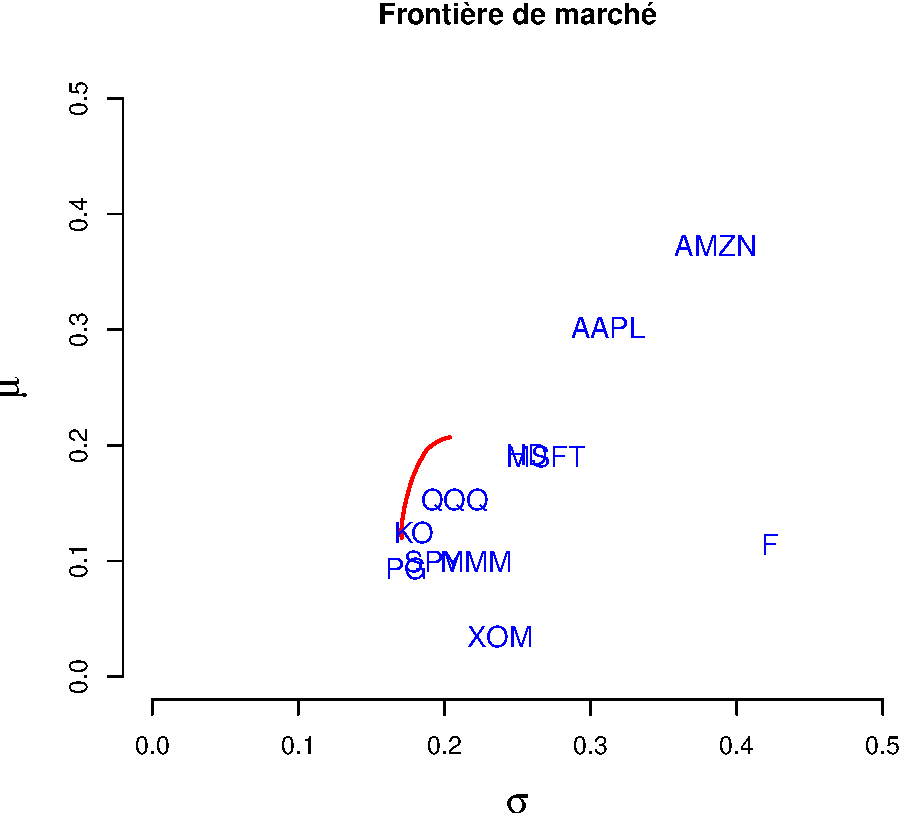
\includegraphics{TP-2_files/figure-latex/unnamed-chunk-18-1.pdf}

\hypertarget{calcul-du-portefeuille-tangent.-1}{%
\subsubsection{Calcul du portefeuille
tangent.}\label{calcul-du-portefeuille-tangent.-1}}

\begin{Shaded}
\begin{Highlighting}[]
\NormalTok{sol.with.rf }\OtherTok{\textless{}{-}} \ConstantTok{NULL}
\ControlFlowTok{for}\NormalTok{(mu.star }\ControlFlowTok{in} \FunctionTok{seq}\NormalTok{(}\AttributeTok{from=}\NormalTok{rf, }\AttributeTok{to=}\FloatTok{1.3}\NormalTok{, }\AttributeTok{length.out=}\DecValTok{200}\NormalTok{))\{}
\NormalTok{  tmp }\OtherTok{\textless{}{-}} \FunctionTok{matrix}\NormalTok{(}\FunctionTok{c}\NormalTok{(mu.star, (mu.star }\SpecialCharTok{{-}}\NormalTok{ rf)}\SpecialCharTok{/}\NormalTok{sharpe.max , sharpe.max, (mu.star }\SpecialCharTok{{-}}\NormalTok{ rf)}\SpecialCharTok{*}\NormalTok{w.tangent), }\AttributeTok{nrow=}\DecValTok{1}\NormalTok{)}
  \ControlFlowTok{if}\NormalTok{(}\FunctionTok{is.null}\NormalTok{(sol.with.rf)) \{}
\NormalTok{    sol.with.rf }\OtherTok{\textless{}{-}}\NormalTok{ tmp  }
\NormalTok{  \} }\ControlFlowTok{else}\NormalTok{ \{}
\NormalTok{    sol.with.rf }\OtherTok{\textless{}{-}} \FunctionTok{rbind}\NormalTok{(sol.with.rf, tmp)}
\NormalTok{  \}}
\NormalTok{\}}
\FunctionTok{dimnames}\NormalTok{(w.tangent)}\OtherTok{\textless{}{-}} \FunctionTok{list}\NormalTok{(tickers)}
\NormalTok{sigma.tangent }\OtherTok{\textless{}{-}} \FunctionTok{sqrt}\NormalTok{(}\FunctionTok{t}\NormalTok{(w.tangent) }\SpecialCharTok{\%*\%}\NormalTok{ Sigma }\SpecialCharTok{\%*\%}\NormalTok{ w.tangent)}
\FunctionTok{colnames}\NormalTok{(sol.with.rf) }\OtherTok{\textless{}{-}} \FunctionTok{c}\NormalTok{(}\StringTok{"mu"}\NormalTok{, }\StringTok{"stdev"}\NormalTok{, }\StringTok{"Sharpe"}\NormalTok{, tickers)}
\FunctionTok{colnames}\NormalTok{(sol) }\OtherTok{\textless{}{-}} \FunctionTok{c}\NormalTok{(}\StringTok{"mu"}\NormalTok{, }\StringTok{"stdev"}\NormalTok{, }\StringTok{"Sharpe"}\NormalTok{, tickers)}
\end{Highlighting}
\end{Shaded}

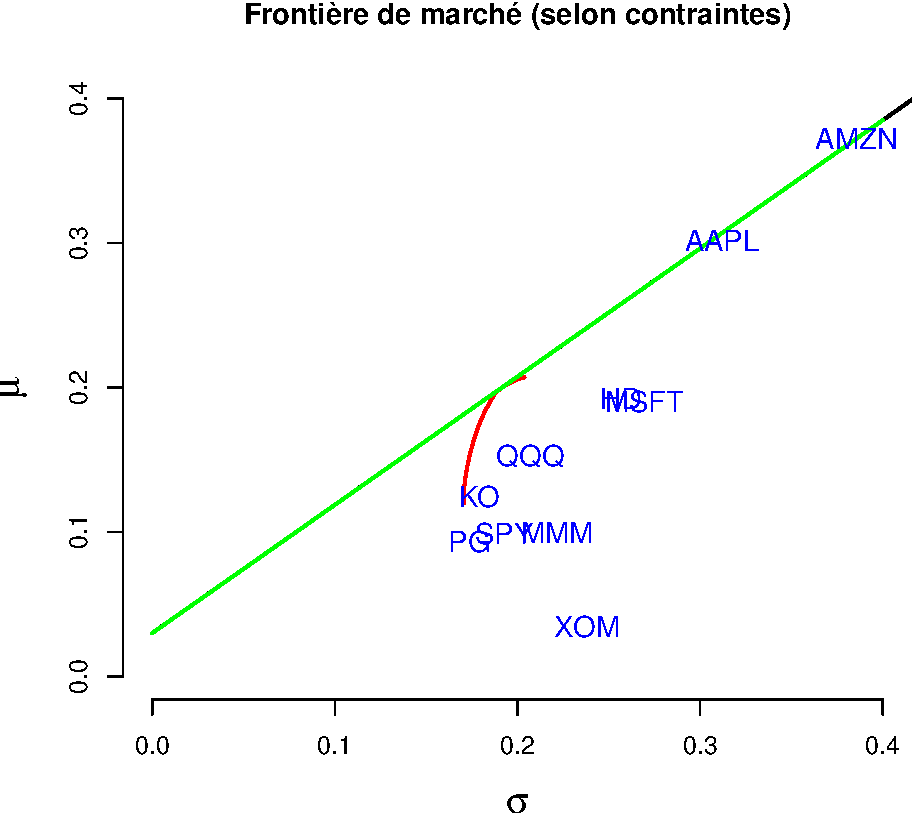
\includegraphics{TP-2_files/figure-latex/unnamed-chunk-20-1.pdf}

\hypertarget{allocation-le-long-de-la-droite-tangente-2}{%
\subsubsection{Allocation le long de la droite
tangente}\label{allocation-le-long-de-la-droite-tangente-2}}

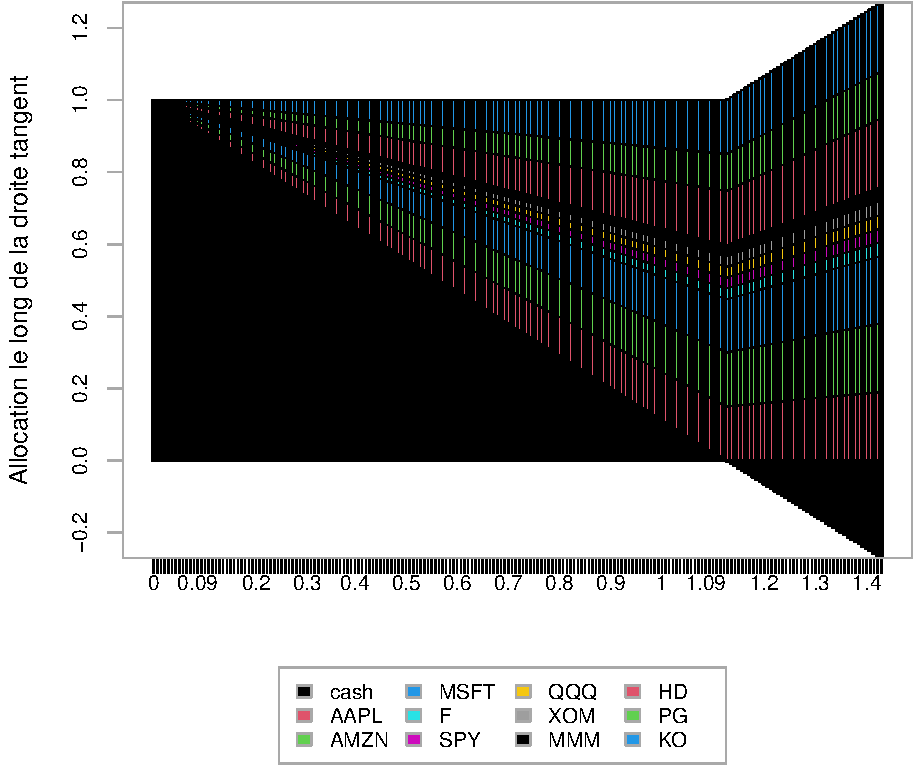
\includegraphics{TP-2_files/figure-latex/unnamed-chunk-21-1.pdf}

\hypertarget{composition-du-portefeuille-tangent-avec-contraintes-1}{%
\subsubsection{Composition du portefeuille tangent avec
contraintes}\label{composition-du-portefeuille-tangent-avec-contraintes-1}}

\begin{Shaded}
\begin{Highlighting}[]
\FunctionTok{kable}\NormalTok{(w.tangent}\SpecialCharTok{*}\DecValTok{100}\NormalTok{, }\AttributeTok{booktabs=}\NormalTok{T, }\AttributeTok{digits=}\DecValTok{2}\NormalTok{, }\AttributeTok{col.names =} \StringTok{"Proportion (\%)"}\NormalTok{,}
      \AttributeTok{caption=}\StringTok{"Composition du portefeuille tangent"}\NormalTok{)}
\end{Highlighting}
\end{Shaded}

\begin{table}

\caption{\label{tab:unnamed-chunk-22}Composition du portefeuille tangent}
\centering
\begin{tabular}[t]{lr}
\toprule
  & Proportion (\%)\\
\midrule
AAPL & 15.00\\
AMZN & 15.00\\
MSFT & 14.72\\
F & 3.00\\
SPY & 3.00\\
\addlinespace
QQQ & 3.00\\
XOM & 3.00\\
MMM & 3.00\\
HD & 15.00\\
PG & 10.28\\
\addlinespace
KO & 15.00\\
\bottomrule
\end{tabular}
\end{table}

\end{document}
